\documentclass[12pt,fleqn]{article}\usepackage{../../common}
\begin{document}
Ders 1

Bu derste matrislerden bahsedilecek, onların canlanmasını, dile gelmesini
isxtiyoruz. Mesela alttaki gibi bir matris

$$ 
K =
\left[\begin{array}{rrrr}
2 & -1 & 0 & 0\\
-1 & 2 & -1 & 0\\
0 & -1 & 2 & -1\\
0 & 0 & -1 & 2
\end{array}\right]
 $$

nedir? Nereden gelir? Bu matris bir şeyi temsil edecek, bilimsel bir
problemi çözmemizi sağlayacak. 

Matrisin özelliklerine bakalım. İlk bakışta bunun simetrik bir matris
olduğunu görüyoruz. Yani $K = K^T$. Bu tür matrisler özellikle dengedeki
sistemler (equilibrium) problemlerinde çok ortaya çıkıyorlar. Başka
özellikler? $K$'yi büyütseydik, seyrek (sparse) olacaktı, yani içinde çok
fazla sayıda sıfır olacaktı. Şu haliyle tam seyrek denemez, ama aynı
kalıpla büyütülürsek seyrek olur. Eğer Python kullanarak sıfır olmayan
elemanları saydırmak isteseydik, sonuç ne gelecekti? 4x4 olan $K$ için
alttaki kod şu sonucu verir,

\begin{minted}[fontsize=\footnotesize]{python}
K = np.array([[2,-1,0,0],[-1,2,-1,0],
              [0,-1,2,-1],[0,0,-1,2]])
print (np.count_nonzero(K))
\end{minted}

\begin{verbatim}
10
\end{verbatim}

4x4 = 16 içinden 10 eleman sıfır değildir. Eğer 100x100 olsaydı? Matris
aynı kalıbı takip ederse, yani çaprazı, ve çaprazın bir altı ve bir üstü
dolu kalırsa, çaprazda 100 eleman olur (boyutla aynı), alt ve üstünde birer
az eleman olur, yani 99+99 = 198. Toplayalım, 100 + 198 = 298. Yani 100x100
= 10000 eleman içinden 298 eleman sıfır değildir, geri kalan bir sürü
eleman sıfırdır. Matris seyrektir.

Sayısal hesaplamada yoğun (dense -sıfırı fazla olmayan-) matrisler, büyük
boyutlarda başımızı ağrıtabilir. Seyrek matrisleri daha hızlı çözmenin
yöntemleri vardır, ama 1 milyon x 1 milyon bir yoğun matris çözmesi imkansız
hale gelebilir.

Başka özellikler? Matris üçlü köşegen (tridiagonal) -üçlü köşegenlik, matris
çaprazı, onun bir üstü ve altı haricindeki tüm diğer elemanların sıfır olduğu
bir matristir-. Bu tür matrisler çok önemlidir, Newton sağolsun, ikinci seviye
diferansiyel denklemlerden sürekli ortaya çıkarlar mesela.

Dahası? Bu bir Toeplitz matrisi, çaprazdaki değerler sabit değerler, çapraz
boyunca hiç değişmiyorlar. Bu matrislere lineer zamana göre değişmeyen
filtreler (linear time invariant filters) ismi de veriliyor, çünkü her
satır birbirinin aynı (ve hesabımızda satırların zamanı temsil ettiği
kabulünden hareketle). Python ile bir Toeplitz yaratmanın yöntemi şöyle:

\begin{minted}[fontsize=\footnotesize]{python}
import scipy.linalg as lin
K = lin.toeplitz([2, -1, 0, 0])
print (K)
\end{minted}

\begin{verbatim}
[[ 2 -1  0  0]
 [-1  2 -1  0]
 [ 0 -1  2 -1]
 [ 0  0 -1  2]]
\end{verbatim}

100x100 için Toeplitz komutuna verdiğimiz tek satırda daha fazla sıfır
gerekli. İçinde tamamen sıfır olan bir vektör yaratırız, başındaki birkaç
elemanı istediğimiz değerle atarız. 

\begin{minted}[fontsize=\footnotesize]{python}
import scipy.linalg as lin
vec = np.zeros((1,100))
vec[0,0] = 2
vec[0,1] = -1
print (lin.toeplitz(vec))
\end{minted}

\begin{verbatim}
[[ 2. -1.  0. ...  0.  0.  0.]
 [-1.  2. -1. ...  0.  0.  0.]
 [ 0. -1.  2. ...  0.  0.  0.]
 ...
 [ 0.  0.  0. ...  2. -1.  0.]
 [ 0.  0.  0. ... -1.  2. -1.]
 [ 0.  0.  0. ...  0. -1.  2.]]
\end{verbatim}

Seyrek matrislerle işlem yaptığımızı Python'a bir şekilde belirtmemiz
lazım, eğer mevcut haliyle bu matrisi çözmeye uğraşırsak, Python sıfırlara
gelene kadar onların sıfır olduğunu bilemeyecektir. 

\begin{minted}[fontsize=\footnotesize]{python}
import scipy.sparse as sparse
import numpy as np
import scipy.linalg as lin
vec = np.zeros((1,100))
vec[0,0] = 2
vec[0,1] = -1
K = lin.toeplitz(vec)
A = sparse.lil_matrix(K)
print (A.shape)
\end{minted}

\begin{verbatim}
(100, 100)
\end{verbatim}

Yanlız yukarıda yoğun matrisi önce yarattım, sonra onu değiştirerek seyrek
matris yarattım, daha iyisi baştan bir seyrek matris yaratmaktı. Neyse, bu
yöntemi ileri de göreceğiz. 

Daha derine inelim şimdi. $K$ matrisi tersi alınabilen (invertible) bir
matris midir? Evet. Bu ne demektir? $KK^{-1} = I$, ve $I$ matrisi birim
(identity) matrisidir, Python'da \verb!np.eye(N)! komutuyla 
yaratılabilir. 

Bir matrisin tersinin alınıp alınamayacağını nasıl anlayabiliriz? Bu çok önemli,
temel bir sorudur.

Bazılarının aklına determinantı hesaplamak gelebilir. Fakat benim ilk
seçimim bu değil, tercihim satır indirgemek (row reduce). Önümüzde bir
matris var, ve içinde neler olup bittiğini bilmiyoruz. Satır indirgeme
yapın.

Bu nasıl yapılır? $K$'in çaprazının altındaki -1 değerlerini sıfırlamak
istiyorum. Orayı temizlemek istiyorum, çünkü matrislerim eğer üçgensel
(triangular) ise, olan biteni anında görebilirim.

Birinci satırı ikiye bölüp, ikinci satıra eklerim. Terminoloji: 0,0 kordinatı
(en üst sol köse) bu işlem sırasında pivot oldu.

$$ 
\left[\begin{array}{rrrr}
2 & -1  &  0 & 0 \\
0 &  3/2 & -1 &  0 \\
0 & -1 & 2 & -1 \\
0 &  0 & -1 & 2 
\end{array}\right]
$$

Şimdi pivot 3/2, ve onun altındaki değeri temizlemek istiyoruz. İkinci
satırın 2/3'ünü alta eklersek, oradaki -1 sıfırlanır.

$$ 
\left[\begin{array}{rrrr}
2 & -1 & 0 & 0 \\
0 & 3/2 & -1 & 0 \\
0 & 0 & 4/3 & -1 \\
0 & 0 & -1 & 2
\end{array}\right]
$$

ve sonunda

$$ 
\left[\begin{array}{rrrr}
2 & -1 & 0 & 0 \\
0 & 3/2 & -1 & 0 \\
0 & 0 & 4/3 & -1 \\
0 & 0 &  0 & 5/4
\end{array}\right]
$$

Bu gerçekten hızlı bir işlem oldu. Python da determinantı zaten böyle
bulacaktı. Yoketme (elimination) kullanacaktı, teker teker -1'leri
yokedecekti. Peki determinantın değeri nedir? 5. Niye 5? Çünkü elimizdeki
artık üçgensel bir matris, ve böyle matrislerde çaprazdaki elemanları
birbiriyle çarpmakla determinant hemen hesaplanır. Python aynen böyle
yapacaktı, $2 \cdot 3/2 \cdot 4/3 \cdot 5/4 = 5$.

Şimdi tersinin olup olmadığı sorusuna geri dönelim: Bir üst üçgensel (upper
triangular) matris ne zaman tersine çevirilebilir haldedir? Determinant
kelimesini kullanmamıza gerek yok, çapraza bakarız, eğer bu çapraz sıfır
değeri olmayan bir çapraz ise bu matris tersine çevirilebilir
demektir. Terminoloji: demek ki elimizde N tane ($K_4$ için 4) tane sıfır
olmayan pivot var. 

1. dersin amaçlarından biri matrislere isim vermek. $K$ matrisi bunlardan
biri, önemli bir matris, onu ileride tekrar göreceğiz, görünce
tanıyacağız. 

$$ 
C = 
\left[\begin{array}{rrrr}
2 & -1 & 0 & -1\\
-1 & 2 & -1 & 0\\
0 & -1 & 2 & -1\\
-1 & 0 & -1 & 2\\
\end{array}\right]
$$

Peki şu matris? Toeplitz formunda ama üst sağ ve alt sol köşelerde ekstra
bir -1 değeri var. Fakat iddia ediyorum ki bu matris tersine çevirebilir
değil ve bunun için determinant, ya da yoketme tekniğine gerek
yok. Terminoloji: Matrise $C$ denilmesi onun değerlerinin dairesel
(circulant) olmasından ileri geliyor. -1 değerlerine bakın, sanki bir
yuvarlak oluşturuyorlar, sıfır değerleri aynı şekilde. 

Devam edelim: Diyelim ki $C$ bir vektörü çarpıyor (zaten matrislerin tek amacı
bu, vektörler ile çarpılmak), ve ortaya sıfır vektörü çıkıyor. Boş olan vektör
ne olabilir?

$$ C = 
\left[\begin{array}{rrrr}
2 & -1 & 0 & -1\\
-1 & 2 & -1 & 0\\
0 & -1 & 2 & -1\\
-1 & 0 & -1 & 2\\
\end{array}\right]
\left[\begin{array}{r}
\\
\\
\\
\\
\end{array}\right]
=
\left[\begin{array}{r}
0\\
0\\
0\\
0
\end{array}\right]
 $$

Şu olabilir

$$ C = 
\left[\begin{array}{rrrr}
2 & -1 & 0 & -1\\
-1 & 2 & -1 & 0\\
0 & -1 & 2 & -1\\
-1 & 0 & -1 & 2\\
\end{array}\right]
\left[\begin{array}{r}
1\\
1\\
1\\
1\\
\end{array}\right]
=
\left[\begin{array}{r}
0\\
0\\
0\\
0
\end{array}\right]
 $$

İddia ediyorum ki böyle bir vektörün olabilmesi $C$'nin tersine çevirilebilir
olma olasılığını yoketti. Nasıl?

Eğer $C$'nin tersi olabilseydi, $Cu = 0$ denklemi ne olurdu? İki tarafı bu
``olabilen'' $C^{-1}$ ile çarpıp sonuca bakalım:

$$ C^{-1}Cu = C^{-1}0 $$

$$ I u = 0 $$

$$ u = 0 $$

Yani eğer $C$'nin tersi olsaydı, $Cu = 0$ denkleminin tek sonucu $u=0$
olurdu. Fakat bu böyle değildir, üstte içinde 1 olan vektör bunun kanıtı. O
zaman bir uyuşmazlık, absürtlük elde ettik, demek ki $C$'nin tersi olduğu
iddiası yanlıştır.

Fiziksel olarak $K$ ve $C$'yi kütle ve yay sistemi olarak kabul
edebiliriz. Mesela $K$ şöyle bir sistemi temsil edebilir:

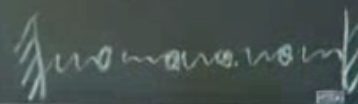
\includegraphics[height=2.5cm]{1_5.png}

Yuvarlak olan $C$ sistemi şunu temsil edebilir

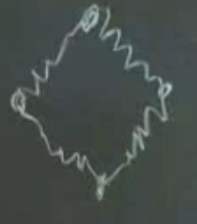
\includegraphics[height=3cm]{1_6.png}

Resimdeki noktalar kütleler, ve yaylar o kütleleri birbirine bağlıyorlar.

$T$ Matrisi

Bu matris $K$'ye benzer, fakat en üst satırda 2 yerine 1 var. 

$$ 
\left[\begin{array}{rrrr}
1 & -1 & 0 & 0\\
-1 & 2 & -1 & 0\\
0 & -1 & 2 & -1\\
0 & 0 & -1 & 2
\end{array}\right]
$$

Kütle ve yay sistemine dönersek bu matris bir ucu serbest olan bir mekanik
sistemi gösterebilir. 

B Matrisi

$$ 
\left[\begin{array}{rrrr}
1 & -1 & 0 & 0\\
-1 & 2 & -1 & 0\\
0 & -1 & 2 & -1\\
0 & 0 & -1 & 1
\end{array}\right]
$$

Bu sistem de her iki ucu da serbest olan bir sistemdir. Bu sistemi alıp
istediğimiz yere götürebiliriz. 

Son iki matrisin ikisi de simetriktir, üçgensel ve köşegen (diagonal)
matrislerdir. Niye üçgensel ve köşegen? Çünkü her kütle sağ ve solunda
tek bir (diğer) kütleye bağlıdır, o yüzden bağlı olmadığı kütlelere olan
matris değeri 0 olarak gösterilir, bu da bir üçgensel köşegen sistem
ortaya çıkarır.

Ama T ve B artık Toeplitz değildir. 

Bu noktada sınır şartları (boundary conditions) kavramına vurgu yapmakta
yarar var. Mekanik sistemde üçün ne olduğu matrislere sınır şartı olarak
yansıyor. Ve bu şartlar bir sistemin çözülmesinde son derece önemli. Hoca
kendisine bir problemle gelenlere genelde ilk önce bu soruyu soruyor o
yüzden: ``sınır şartların ne?''. 

Tersine çevirilme durumu? T tersine çevirilebilir, B çevirilemez. B için
yine aynı
$u = \left[\begin{array}{cccc} 1 & 1 & 1 & 1 \end{array}\right]^T$ ispatını
kullanabiliriz.

K, T, B, C matrislerini aynı anda yaratan bir Python programı
şurada. Kullanım mesela 4x4 boyutları için \verb!K, T, B, C = ktbc(4)!
şeklinde, bu bize tüm özel matrisleri bir kerede oluşturuyor.

\begin{minted}[fontsize=\footnotesize]{python}
import scipy.linalg as lin

def ktbc(n):
    vec = np.zeros((1,n))
    vec[0,0] = 2
    vec[0,1] = -1
    K = lin.toeplitz(vec)
    T = np.copy(K)
    T[0,0] = 1
    B = np.copy(K)
    B[0,0] = 1
    B[n-1,n-1] = 1
    C = np.copy(K)
    C[n-1,n-1] = 1
    
    return K, T, B, C
\end{minted}

Kapatırken şu özellikleri de ekleyelim. 

K, T pozitif kesin (positive definite) matrislerdir. 

C, B pozitif yarı-kesin (positive semi-definite) matrislerdir. 

Eğer simetrik bir matrisim var ise ve pivotların hepsi pozitif ise, o
matris hem tersine çevirelebilir, hem de pozitif kesin demektir. Yani bir
matrise bakarız, yoketme tekniğini uygularız sonra pivotlarına bakarız. 

Pozitif kesinlik çok önemli bir kavramdır, lineer cebirin tamamını biraraya
getirir sanki, özdeğerlere (eigenvalue) bağlıdır, least square yöntemine
bağlıdır, determinantlar. Her yerden çıkar. 

Geriye Doğru Farklılık Matrisi

Python \verb!toeplitz! çağrısının değişik bir şekilde kullanarak geriye
doğru farklılık (backward difference) matrisi de yaratabiliriz. Bu
kullanımda matrisin sol kolonunu, ve üst satırını tamamen belirtmek
gerekiyor.

\begin{minted}[fontsize=\footnotesize]{python}
import scipy.linalg as lin

D = lin.toeplitz([1, -1, 0, 0], [1, 0, 0, 0])
print (D)
\end{minted}

\begin{verbatim}
[[ 1  0  0  0]
 [-1  1  0  0]
 [ 0 -1  1  0]
 [ 0  0 -1  1]]
\end{verbatim}

Çözülmüş Soru 1.1 B

Soru: $T$ matrisini $H$ matrisine çevir bunu $J$ matrisini kullanarak
yap. 

$$ H = 
\left[\begin{array}{rrr}
2 & -1 &  0\\
-1 & 2 & -1\\
0 & -1 & 1
\end{array}\right]
 $$

$$ T = 
\left[\begin{array}{rrr}
1 & -1 &  0\\
-1 & 2 & -1\\
0 & -1 & 2
\end{array}\right]
 $$

Kitaptaki bu sorunun çözümündeki $J$ matrisi birimsel matrisin tersidir, 
şu şekildedir:

$$ 
\left[\begin{array}{rrr}
0 & 0 & 1\\
0 & 1 & 0\\
1 & 0 & 0
\end{array}\right]
 $$

Yani 1 sayıları sola yatık çaprazda değil sağa yatik çaprazda. Bu matrisin
çarpım işlemi sırasında ilginç etkileri var. Eğer sağdan çarpılırsa bir
matrisin her satırının içindeki sırayı tersine çeviriyor. Eğer soldan
çarpılırsa her kolon içindeki sırayı tersine çeviriyor. $J*T*J$ çarpımı
aradığımız sonuç. Yani satırları çevirdikten sonra, kolonları çevirince
istediğimiz sonuca erişiyoruz. Python kodları

\begin{minted}[fontsize=\footnotesize]{python}
import scipy.linalg as lin
T = lin.toeplitz([2, -1, 0])
T[0,0] = 1
J = np.fliplr(np.eye(3))
print (T)
print (np.dot(T,J))
print (np.dot(J, np.dot(T,J)))
\end{minted}

\begin{verbatim}
[[ 1 -1  0]
 [-1  2 -1]
 [ 0 -1  2]]
[[ 0. -1.  1.]
 [-1.  2. -1.]
 [ 2. -1.  0.]]
[[ 2. -1.  0.]
 [-1.  2. -1.]
 [ 0. -1.  1.]]
\end{verbatim}

Soru 1.1 2

$T_3^{-1}$ hesabını üç basamakta yap ve bunu yaparken daha önce gördüğümüz
$U$ ve $U^{-1}$ matrislerini kullan.

\begin{minted}[fontsize=\footnotesize]{python}
import scipy.linalg as lin

T = lin.toeplitz([2, -1, 0])

T[0,0] = 1

U = np.array([[1, -1, 0],
              [0, 1, -1],
              [0, 0, 1]])

print (np.dot(U.T,U))
print (np.dot(U,lin.inv(U)))
print (np.dot(lin.inv(U), lin.inv(U).T))
\end{minted}

\begin{verbatim}
[[ 1 -1  0]
 [-1  2 -1]
 [ 0 -1  2]]
[[1. 0. 0.]
 [0. 1. 0.]
 [0. 0. 1.]]
[[3. 2. 1.]
 [2. 2. 1.]
 [1. 1. 1.]]
\end{verbatim}

Soru 1.1.5

$K_3$ ve $K_4$'un tersini al ($K_2$'yi de bir zahmet), ve şu kesirler olsun

$$ \frac{1}{det} = \frac{1}{4} \frac{1}{5}$$. 

$$
K_3^{-1} = \frac{1}{4}
\left[\begin{array}{rrr}
3 & 2 & 1 \\
2 & 4 & 2 \\
1 & 2 & 3
\end{array}\right]
\quad \textrm{ve} \quad
K_4^{-1} = \frac{1}{5}
\left[\begin{array}{rrrr}
4 & 3 & 2 & 1 \\
3 & 6 & 4 & 2 \\
2 & 4 & 6 &  3 \\
1 & 2 & 3 & 4
\end{array}\right]
$$


İlk önce $K=K_5$ determinantını tahmin edin. Sonra $\det(K)$ ve
$inv(K)$'yi hesaplayın ve $\det(K) * inv(K)$ hesabını yapın. 

\begin{minted}[fontsize=\footnotesize]{python}
import scipy.linalg as lin

K, T, B, C = ktbc(3)
print (lin.inv(K))
print (lin.det(K))
print (lin.det(K) * lin.inv(K))

K, T, B, C = ktbc(5)
print (lin.det(K))
print (lin.inv(K))
print (lin.det(K) * lin.inv(K))
\end{minted}

\begin{verbatim}
[[0.75 0.5  0.25]
 [0.5  1.   0.5 ]
 [0.25 0.5  0.75]]
4.0
[[3. 2. 1.]
 [2. 4. 2.]
 [1. 2. 3.]]
6.0
[[0.83333333 0.66666667 0.5        0.33333333 0.16666667]
 [0.66666667 1.33333333 1.         0.66666667 0.33333333]
 [0.5        1.         1.5        1.         0.5       ]
 [0.33333333 0.66666667 1.         1.33333333 0.66666667]
 [0.16666667 0.33333333 0.5        0.66666667 0.83333333]]
[[5. 4. 3. 2. 1.]
 [4. 8. 6. 4. 2.]
 [3. 6. 9. 6. 3.]
 [2. 4. 6. 8. 4.]
 [1. 2. 3. 4. 5.]]
\end{verbatim}

Soru 1.1.22

Çözülmesi istenen denklem $du^2/dx^2 = 1$, elastik çubuk problemi ve
çubuğun iki tarafı sabitlenmiş.

\begin{minted}[fontsize=\footnotesize]{python}
import scipy.sparse as sparse
import scipy.sparse.linalg
import scipy.linalg as lin

n = 1000
vec = np.zeros((1,n))
vec[0,0] = 2; vec[0,1] = -1
K = lin.toeplitz(vec)
A = sparse.csc_matrix(K)
e = np.ones((n,1))

u = sparse.linalg.spsolve(A,e)
plt.plot(u)
plt.savefig('1-1-22.png')
\end{minted}

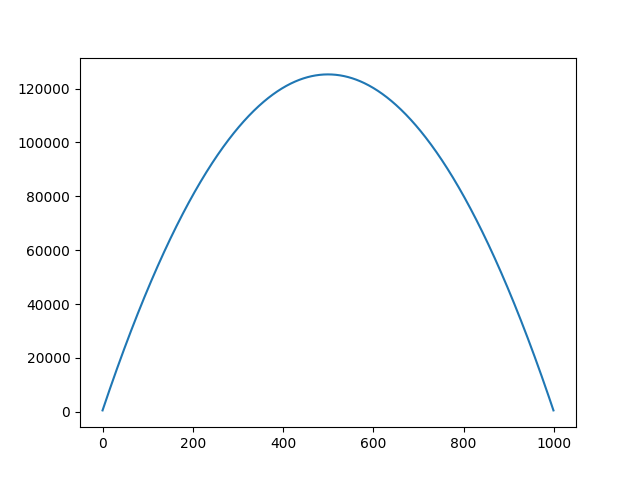
\includegraphics[height=5cm]{1-1-22.png}

Sonuç üstteki grafik gibi olmalı. Yani çözümümüz olan $u$ değerleri bir parabol
oluşturuyorlar. Bu demektir ki çubuğun orta noktaları daha fazla yer
değiştiriyor, uç noktaları daha az yer değiştiriyor.

Elastik Çubuk

Derste çokça kullanılan elastik çubuk kavramından şimdi bahsetmek iyi olur. Bu
çubuk tek boyutlu ve sadece boyuna doğru (yana doğru değil) uzayıp kısalabilen
matematiksel bir kurgu. Bu çubuğu hayalimizde birbirine zincirler ile bağlı
sonsuz sayıda ufak parcaçığın toplamı olarak düşünebiliriz. $x$ ve $u(x)$
bağlamında ise çubuğun iki kere fotoğrafının çekildiğini düşünelim. İlk
fotoğrafta $x$ bu çubuğun üzerindeki bir parcaçık. $u(x)$ ise tüm ağırlıklar,
kuvvetler etkilerini gösterip uzama, kısalma bitince çekilen {\em ikinci}
fotoğrafta ilk resimdeki $x$ noktasının ne kadar yer değiştirmiş olduğu.

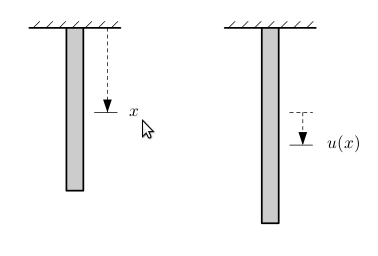
\includegraphics[height=4cm]{1_7.png}

``Ucu sabitlemek'' gibi kavramlar duyacağız, bunlar bazen fiziksel olarak
anlamlı, bazen ise ikinci fotoğrafta esneme sonrası hangi noktaya
gelindiğinin önceden belirlenmesi anlamında. $du/dx$ gibi bir türevi
irdelerken ise ortada zaman olmadığını dikkate alalım, türev $x$'e göre
yani ilk resimdeki parcaçıgin yeri. O zaman $du/dx$ ikinci resimdeki
esnemenin çubuktaki yer arttıkça (aşağı indikçe) ne kadar değiştiği. 

Denklemin sağında yer alan değerler, sisteme dışarıdan verilen güç olarak
görülebiliyor, hakikaten de değişimin ikinci türevi ivmedir. 1.2.22 sorusunu
görsel olarak nasıl hayal edebiliriz? Çubuğun iki ucu sabitlenmiş, o sebeple K
matrisi kullanıyoruz zaten, böylece sınır şartları dahil oluyor.

Python, VPython üzerinden kullanılabilecek KineticsKit adlı paket sistemi
zihinde canlandırmak için yardımcı olabilir. Birbirine eşit uzaklıkta, aynı
kütlede ve arasında yaylar olan 7 tane topu bırakınca ne olduğunu simüle
edebiliriz. Resimdeki sol kısım başlamadan önce, sağ kısım yerçekimi işini
bitirdikten ve toplar durduktan sonrasını gösteriyor.

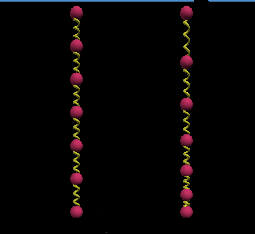
\includegraphics[height=5cm]{elastic_uniform_load.png}

Alttaki program hem görsel simülasyonu yapacak, hem de topların önce ve
sonra değerlerini hatırlayarak yerçekimi sonrası aradaki farkı
hesaplayacak. Sonuçlara bakınca hakikaten de ortadaki topların daha fazla
hareket ettiğini görebiliyoruz. Grafiksel olarak düşünürsek te mantıklı,
üste yakın toplar üstten bağlı oldukları için fazla uzaklaşamıyorlar,
ortalara yakın toplar, bir üstlerinden de aldıkları ek mesafe sayesinde
daha fazla yer değiştirebiliyor. Ama alt kısıma yaklaştıkça orada bir
birikme oluyor, çünkü alt üç kısım da sabitlenmiş. 

\inputminted[fontsize=\footnotesize]{python}{elastic_uniform_load.py}


\end{document}
